\chapter{Registros de actividad neuronal}\label{cha:neuro}

Finalmente, en este capítulo analizaremos los registros de actividad neuronal adquiridos durante la ejecución de la tarea \textit{rotarod} con aceleración. Estos registros electrofisiológicos fueron adquiridos en la región locomotora del mesencéfalo (MLR) de los ratones expertos en la tarea \textit{rotarod}. El MLR es una región del mesencéfalo asociada a los procesos de iniciación y de control de la velocidad en la locomoción \cite{caggiano_midbrain, roseberry_locomotor, shik_walking}. Esta región se comunica río abajo con la médula espinal y es necesaria para el proceso de locomoción \cite{nielsen_mlr_walk, capaday_mlr_walk}. Lesiones o patologías en los núcleos de esta región pueden ocasionar ataxia y falta de coordinación en la locomoción \cite{hathout_ataxia}. En esta parte del trabajo nos preguntamos si la actividad de algunas de las neuronas presentes en esta región del cerebro estaría modulada por el movimiento del ratón en el transcurso de la tarea \textit{rotarod} \cite{skinner_mlr_rat, sherman_mlr_cat, leray_mlr_vertebrate}. Para contestar esta pregunta estudiaremos correlaciones entre la actividad neuronal y la ocurrencia de transiciones de poses.

A continuación, una breve descripción del contenido de este capítulo. Primero, en la Sección \ref{sec:sorting} describiremos el algoritmo de \textit{spike sorting} utilizado para extraer información sobre los tiempos de disparo de las neuronas a partir de las señales registradas por los electrodos. Después, estudiaremos si la actividad de las neuronas registradas está modulada por la ocurrencia de eventos de transiciones de poses. Por un lado, en la Sección \ref{sec:neurona} mostraremos algunos patrones típicos de disparo para neuronas individuales. Por otro lado en la Sección \ref{sec:poblacion} mostraremos los patrones de actividad de conjuntos de varias neuronas, ante la ocurrencia de un evento de transición de poses.

\section{Registro de actividad de neuronas individuales}\label{sec:sorting}

Se utilizaron implantes crónicos de sondas de silicio (\textit{silicon probes}) conteniendo 16 electrodos para registrar la actividad eléctrica de neuronas del MLR de los ratones durante la ejecución de la tarea \textit{rotarod} (Figura \ref{fig:mlr}). La sonda de silicio fue montada sobre una guía que permite cambiar la profundidad de la sonda de manera precisa. Durante la sesión de registro de la actividad neuronal los electrodos fueron conectados a un \textit{headstage} que  contenía un conjunto de 16 amplificadores operacionales. A su vez, el \textit{headstage} estaba conectado a un preamplificador de 16 canales \cite{esposito_defensive} que envía la información a la tarjeta de adquisición que sincroniza las señales eléctricas con la información adquirida a través de las cámaras de video.

\begin{figure}[!htbp]
    \centering
    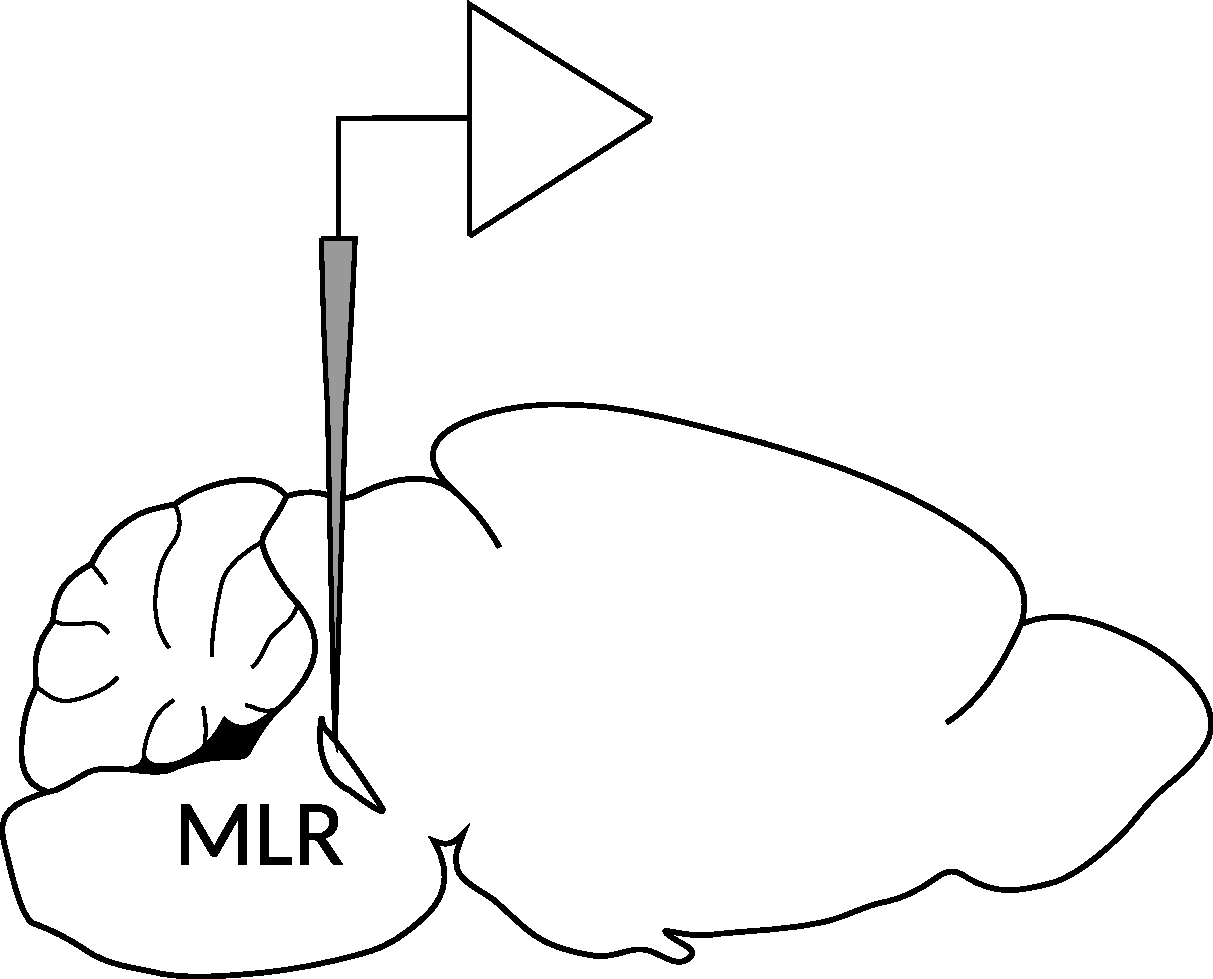
\includegraphics[width=0.3\linewidth]{figuras/cerebro/mlr.pdf}
    \caption{Esquema de la ubicación del arreglo de electrodos para el registro electrofisiológico de neuronas en el MLR.}
    \label{fig:mlr}
\end{figure}

Se digitalizaron las señales de actividad neuronal a una frecuencia de muestreo de 40 kHz, y se le aplicó un filtro pasa-banda en el rango de 250 Hz a 8 kHz. La señal se pre-procesó utilizando el sistema de adquisición \textit{Neural Recording Data Acquisition System} (Omniplex, Plexon). Finalmente, utilizando el programa \textit{Offline Sorter} (OFS, Ominplex, Plexon) se descompuso la señal electrofisiológica multicanal adquirida en disparos de neuronas individuales. El programa OFS es una implementación de un algoritmo de \textit{spike sorting} supervisado, que identifica \textit{clusters} en las componentes principales de la señal con la actividad de neuronas individuales. Luego, se realizan análisis de correlación cruzada y de auto correlación para corroborar que la identidad de las neuronas identificadas sea única e individual. Es decir, se corrobora que no haya neuronas duplicadas y que no haya neuronas multi-unidad que estén compuestas por las actividades de más de una única neurona \cite{esposito_defensive}.

\section{Actividad de neuronas individuales}\label{sec:neurona}

\begin{figure}[!htbp]
\centering
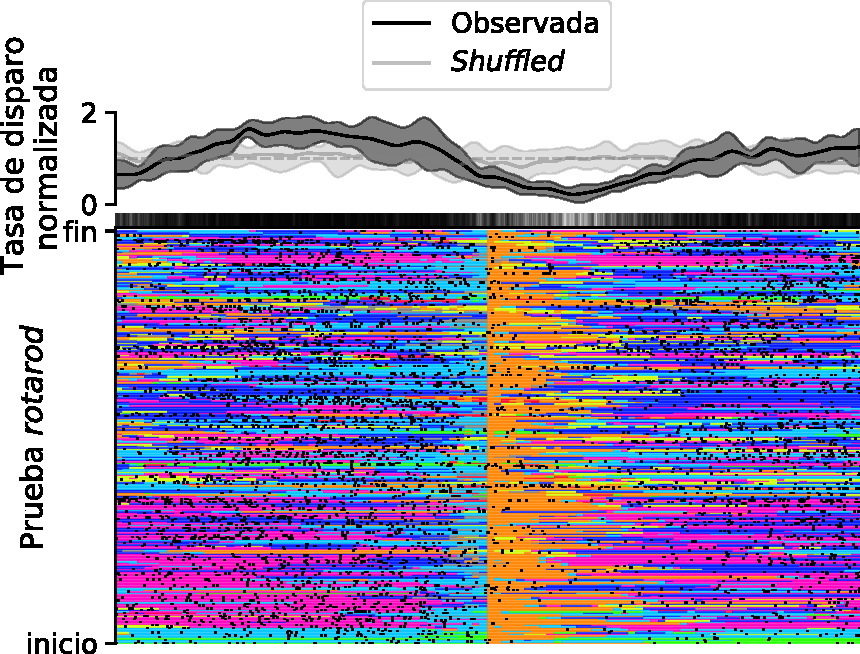
\includegraphics[width=0.67\textwidth]{figuras/expertos/disparo/raster_mouse3_day10_trial08_label2_neuronSPKC11a.pdf}
\vspace{1em}
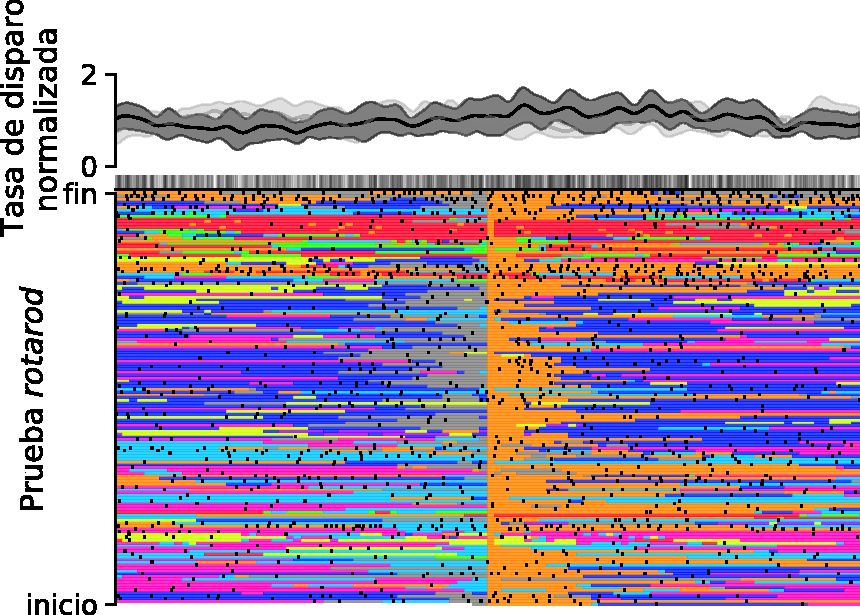
\includegraphics[width=0.67\textwidth]{figuras/expertos/disparo/raster_mouse3_day04_trial08_label2_neuronSPKC11a.pdf}
\vspace{1em}
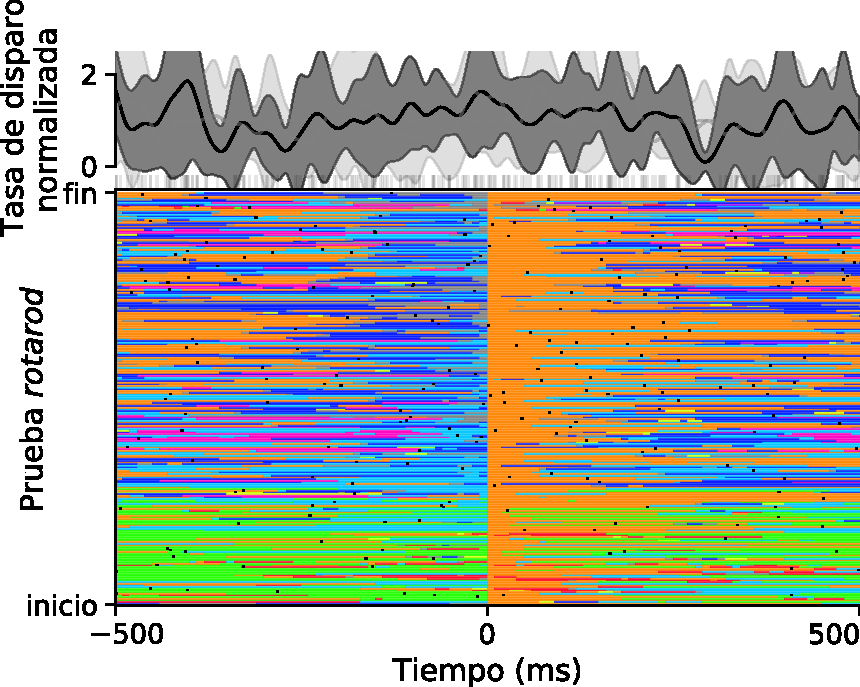
\includegraphics[width=0.67\textwidth]{figuras/expertos/disparo/raster_mouse3_day05_trial10_label2_neuronSPKC09a.pdf}
\caption{Diferentes patrones de actividad neuronal registrados alrededor de un tipo de evento de transición entre poses clasificadas (en este caso, el evento es una transición hacia el \textit{label} 2). Tasas de disparo normalizadas y \textit{raster plots} para tres neuronas diferentes, cada una durante una prueba \textit{rotarod} distinta. Los intervalos de error de las tasas de disparo se obtuvieron mediante \textit{bootstrapping}.}
\label{fig:disparos_label2}
\end{figure}

Con el fin de comprender si las neuronas del MLR codifican de alguna manera la información de la pose del animal, decidimos realizar un gráfico de raster de la actividad neuronal alineado al inicio de cada pose para cada neurona registrada durante cada ensayo individual. La Figura \ref{fig:disparos_label2} muestra los patrones de disparo de tres neuronas representativas. Habiendo alineado la actividad neuronal a la ocurrencia de un evento determinado, puede estudiarse la distribución de disparos de la neurona en una ventana de tiempo alrededor del evento. Para ello, se utilizó un KDE gaussiano, con un \textit{bandwidth} de 20 ms, para estimar la tasa de disparo (\textit{firing rate}) de las neuronas alrededor de la ocurrencia de un evento. Esto se implementó en Python usando la clase \texttt{gaussian\_kde} de \texttt{scipy.stats} \cite{scipy}. Esta tasa de disparo se normaliza para que la cantidad total de disparos sea la misma para todas las neuronas. De esta manera, se facilita la comparación de las neuronas de baja actividad con las neuronas de alta actividad. En términos formales, si $f(t)$ denota el \textit{firing rate} de una neurona en torno a un determinado evento, entonces el \textit{firing rate} normalizado $\tilde{f}(t)$ se obtiene de la siguiente manera
\begin{equation}
    \tilde{f}(t) = \frac{f(t)}{\int_{a}^{b} f(t) \dd{t}},
\end{equation}
donde $[a, b]$ es el intervalo de tiempo estudiado alrededor de la ocurrencia del evento. 

En nuestro caso, estudiaremos ventanas de tiempo de [$-500$, 500] ms alrededor de la ocurrencia de un evento. En particular, consideraremos dos grupos de eventos de transición entre poses: transiciones que salen de un determinado \textit{label} $l$ (evento que denominaremos \textit{offset} del \textit{label $l$}) y transiciones que llegan a un determinado \textit{label} (\textit{onset} del \textit{label} $l$).

Además de la tasa de disparo normalizada observada alrededor de la ocurrencia de un evento, la Figura \ref{fig:disparos_label2} muestra también una tasa de disparo de referencia, obtenida luego de intercambiar aleatoriamente los tiempos de disparo de la neurona. Llamaremos a esta tasa de disparo de referencia ``\textit{shuffled}''. Dentro de la ventana de tiempo alrededor de la ocurrencia de un evento, la tasa de disparo \textit{shuffled} se calcula permutando los tiempos de disparo de la neurona, bajo la condición de conservar los intervalos de tiempo inter-disparo y el número total de disparos.

Finalmente, en la Figura \ref{fig:disparos_label2} se muestran eventos de transición del tipo \textit{onset} del \textit{label} 2. Recordemos que este \textit{label} está asociado a una pose en la que el ratón da un paso con su pata derecha sobre el cilindro \textit{rotarod}. Para cada prueba \textit{rotarod} que se muestra en la Figura \ref{fig:disparos_label2} se utiliza el mismo código de colores del etograma de la Figura \ref{fig:tsne_labels} para indicar la ocurrencia de diferentes \textit{labels}. A su vez, se indican los eventos de disparo de la neurona con marcadores negros (\textit{raster plot}). En la parte superior de cada prueba \textit{rotarod} se muestra el \textit{firing rate} normalizado observado (línea continua negra) y la referencia \textit{shuffled} (línea continua gris). Además se muestra el valor teórico constante de \textit{firing rate} completamente aleatorio y no correlacionado con el evento (línea discontinua gris). Los intervalos de error que se muestran para el \textit{firing rate} se calcularon utilizando un esquema de \textit{bootstraping} con los tiempos de disparo alrededor de la ocurrencia del evento de transición. Este intervalo de error sirve para comparar la relevancia de la modulación del \textit{firing rate} observado frente al \textit{shuffled}.
Por último, puede observarse que algunas neuronas están marcadamente moduladas ante la ocurrencia del evento de transición (Figura \ref{fig:disparos_label2}, panel superior), otras están levemente moduladas (Figura \ref{fig:disparos_label2}, panel medio)y otras neuronas no están moduladas de manera significativa al compararla con la tasa de disparo \textit{shuffled} (Figura \ref{fig:disparos_label2}, panel inferior).

\section{Patrones de actividad de grupos de neuronas}\label{sec:poblacion}

Cabe mencionar que se cuenta con registros de la actividad neuronal a lo largo de diferentes días y cada día consiste en un promedio de 3 a 4  pruebas de \textit{rotarod} por ratón. Con el fin de determinar cuáles neuronas están moduladas por las poses adoptadas por el animal mientras realiza la tarea \textit{rotarod}, tomaremos estos conjuntos de observaciones de una misma neurona en diferentes pruebas de un mismo día y promediaremos sus tasas de disparo en torno a la ocurrencia de un determinado evento de transición. Es importante destacar que consideraremos que los registros de actividad neuronal provienen de diferentes neuronas día tras día, pues la posición del arreglo de electrodos se modificaba cada día alrededor de \SI{50}{\micro\metre} para aumentar el tamaño de la muestra de neuronas registradas. 

Para cada una de estas tasas de disparo promedio $\bar{f}(t)$ por neurona, calcularemos el correspondiente \textit{z-score}, definido como:
\begin{equation}
    z(t) = \frac{\bar{f}(t) - \mu_{\bar{f}}}{\sigma_{\bar{f}}},
\end{equation}
donde $\mu_{\bar{f}}$ y $\sigma_{\bar{f}}$ son el valor medio y la desviación estándar de la tasa de disparo promedio $\bar{f}(t)$ para las observaciones de neurona en particular, ante la ocurrencia de un determinado evento de transición entre poses. Por lo tanto el valor del \textit{z-score} $z(t)$ indica cuántos desvíos estándares se aleja la actividad de la neurona en un determinado tiempo $t$, respecto del valor medio de la actividad de la neurona $\mu_{\bar{f}}$.

Utilizar el \textit{z-score} nos permite comparar la actividad entre diferentes neuronas con facilidad. Por su parte, podemos agrupar neuronas según qué tan moduladas están ante la ocurrencia de un evento. Para determinar cuantitativamente cuándo la actividad de una neurona está modulada o no ante la ocurrencia de un evento de transición se utiliza la prueba de Kolmogorov-Smirnov (\textit{test} KS). Para ello, se utilizó la función \texttt{ks\_2samp} de \texttt{scipy.stats} \cite{scipy}, implementada en Python. A través del \textit{test} KS se comparan las distribuciones del \textit{firing rate} promedio $\bar{f}(t)$ observado con el \textit{shuffled firing rate} promedio de una neurona. Si los valores de ambas tasas de disparo tienen la misma distribución de probabilidad entonces consideraremos que la actividad de la neurona no está modulada por la ocurrencia del evento de transición.

Utilizando el \textit{test} KS, consideraremos que dos muestras de variables aleatorias tienen la misma distribución de probabilidad cuando el valor del estadístico del \textit{test} sea menor a 0.2 y su p-valor sea mayor a 0.05. La hipótesis nula del \textit{test} KS es que ambas variables aleatorias provienen de la misma distribución de probabilidad. Además, si solo el valor del estadístico es menor a 0.2 o si solo el p-valor es mayor a 0.05 consideraremos que no podemos rechazar la hipótesis nula. Por lo tanto, ambas variables aleatorias provendrían de la misma distribución de probabilidad. De esta manera, concluiremos que la actividad de la neurona no está modulada por la ocurrencia del evento, dado que los valores que adopta el \textit{firing rate} observado y el \textit{shuffled firing rate} son indistinguibles.

Por el contrario, si se satisface que el estadístico del \textit{test} KS sea mayor a 0.2 y que el p-valor sea menor a 0.05 entonces consideraremos que ambas variables aleatorias tienen distribuciones de probabilidad diferentes. En nuestro caso, esto significa que los valores del \textit{firing rate} observado y del \textit{shuffled firing rate} tienen distribuciones diferentes. Concluyendo, de esta manera, que la actividad de la neurona sí está modulada por la ocurrencia del evento de transición de poses.

Las Figuras \ref{fig:zscore_label2}, \ref{fig:zscore_label5}, \ref{fig:zscore_label6} y \ref{fig:zscore_label7} muestran los patrones de actividad de grupos de neuronas ante la ocurrencia de eventos de \textit{onset} y \textit{offset} de los \textit{labels} 2, 5, 6 y 7, respectivamente (los patrones de actividad para los \textit{labels} 1, 3, 4, 8 y 9 se muestran en el Apéndice \ref{cha:popu_cont}). Estos patrones de actividad neuronal consisten en \textit{heatmaps} con los valores de \textit{z-score} de cada una de las neuronas observadas. Cada fila en el \textit{heatmap} representa una neurona individual. El tiempo de ocurrencia del evento se indica con una línea discontinua negra vertical. Además, estos \textit{heatmaps} presentan una división entre neuronas no moduladas y moduladas ante la ocurrencia del evento de transición (línea continua negra horizontal).

A su vez, cada uno de estos grupos de neuronas se ordena de tres maneras diferentes para facilitar su visualización: pueden estar ordenados según la posición del máximo o del mínimo de su \textit{z-score} o según un orden por defecto. Al ordenar los \textit{z-scores} de las neuronas no moduladas, según las posiciones de sus máximos o mínimos, esperamos observar un patrón de alineamiento sobre la diagonal del \textit{heatmap} del grupo (esta diagonal se indica con una línea discontinua gris tanto para las neuronas no moduladas como para las neuronas moduladas). Esto se debe a que si las neuronas no están moduladas por la ocurrencia del evento, entonces sus valores de \textit{z-score} serían completamente aleatorios y la posición de su valor máximo o mínimo seguiría una distribución de probabilidad uniforme en la ventana de tiempo analizada. De esta manera, se esperaría que los máximos o mínimos de las neuronas no moduladas estén alineados sobre la diagonal.

Por su parte, se espera que los máximos y mínimos de las neuronas que sí están moduladas presenten desviaciones respecto de la diagonal del \textit{heatmap}, ya que estarían correlacionadas de alguna manera con la ocurrencia del evento de transición. También sería razonable esperar que estas neuronas puedan subdividirse en grupos que responden a la ocurrencia del evento con tiempos característicos similares o con patrones de disparo similares. Cabe mencionar que en nuestro experimento alrededor de un tercio (32\% a 33\%) de las neuronas registradas veían su actividad modulada por transiciones involucrando al \textit{label} 2, mientras que para los \textit{labels} 5, 6 y 7 la fracción de neuronas con actividad modulada fue de un quinto a un cuarto de las neuronas registradas (entre 20\% y 24\%).

\begin{figure}[!htbp]
\begin{tabular}{clll}
& & \multicolumn{2}{c}{\hspace{-5.5em} \textit{Label} 2} \\
& & \hspace{6em} \textit{Onset} & \hspace{6em} \textit{Offset} \\
\rotatebox[origin=c]{90}{Orden según máximo} & \rotatebox{90}{\hspace{-8.5em} Moduladas \hspace{2.5em} No moduladas} & \raisebox{-0.5\height}{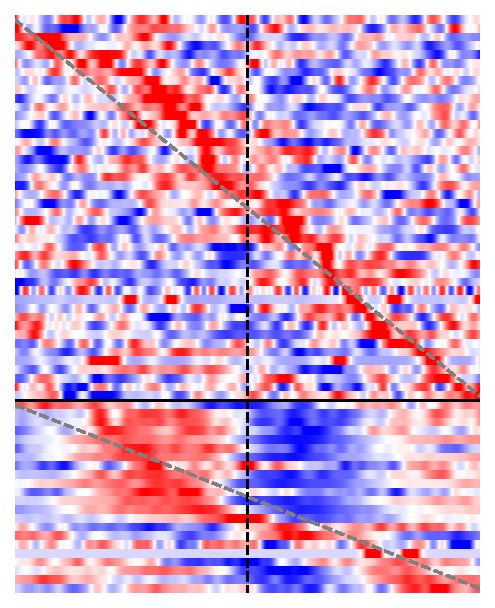
\includegraphics[width=0.37\textwidth]{figuras/expertos/zscore/rasters_separate_days_zscore_max_onset_label2.pdf}} &
\raisebox{-0.5\height}{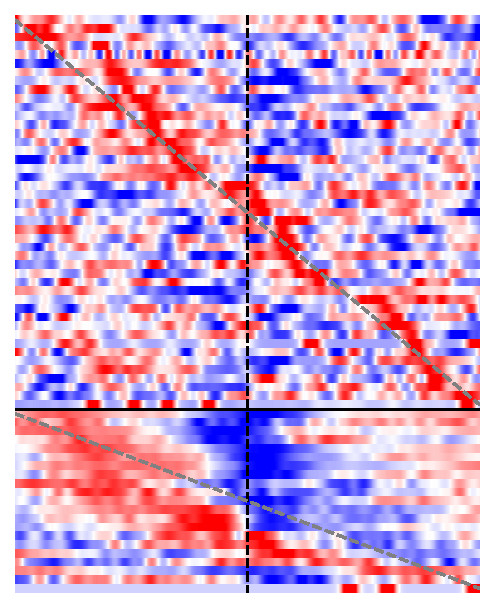
\includegraphics[width=0.37\textwidth]{figuras/expertos/zscore/rasters_separate_days_zscore_max_offset_label2.pdf}} \\
\rotatebox[origin=c]{90}{Orden según mínimo} & & \raisebox{-0.5\height}{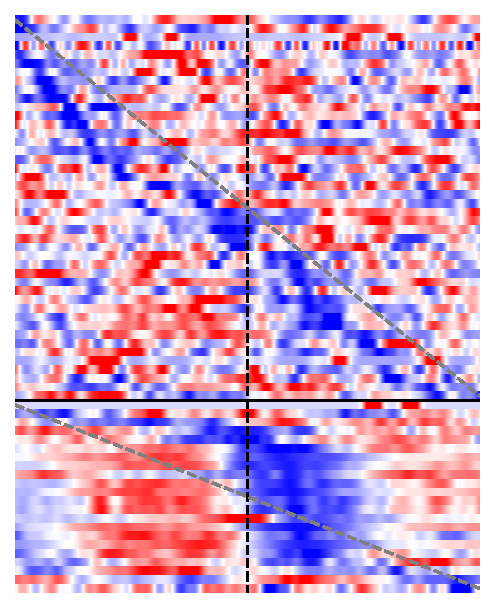
\includegraphics[width=0.37\textwidth]{figuras/expertos/zscore/rasters_separate_days_zscore_min_onset_label2.pdf}} &
\raisebox{-0.5\height}{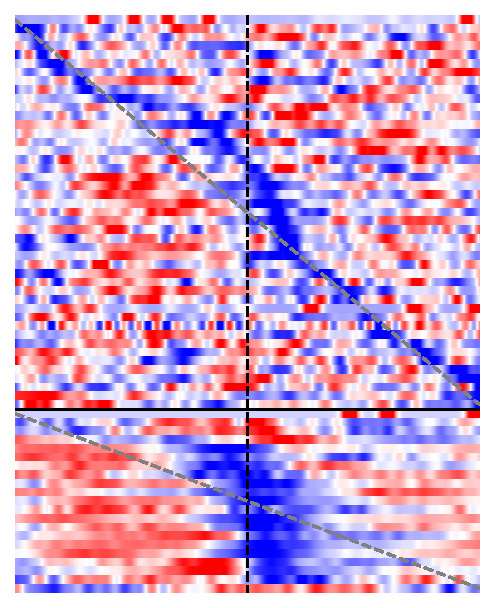
\includegraphics[width=0.37\textwidth]{figuras/expertos/zscore/rasters_separate_days_zscore_min_offset_label2.pdf}} \\
\rotatebox{90}{Orden por defecto} & & \hspace{-1.5em} \raisebox{-0.5\height}{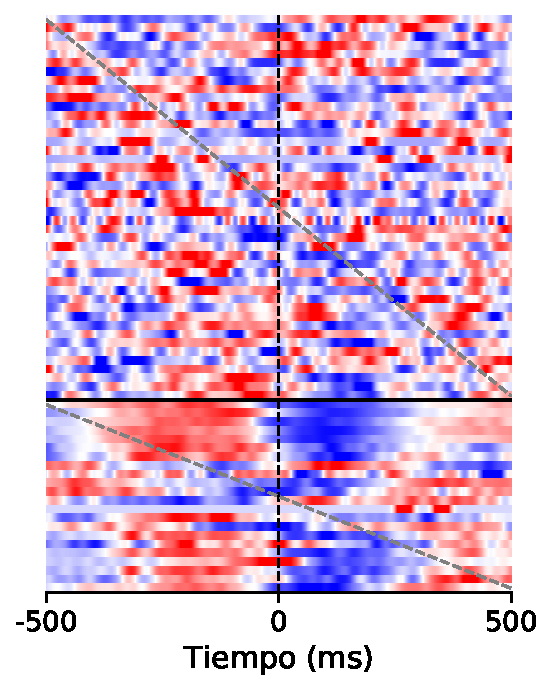
\includegraphics[width=0.42\textwidth]{figuras/expertos/zscore/rasters_separate_days_zscore_deafult_onset_label2.pdf}} & \hspace{-1.3em} \raisebox{-0.495\height}{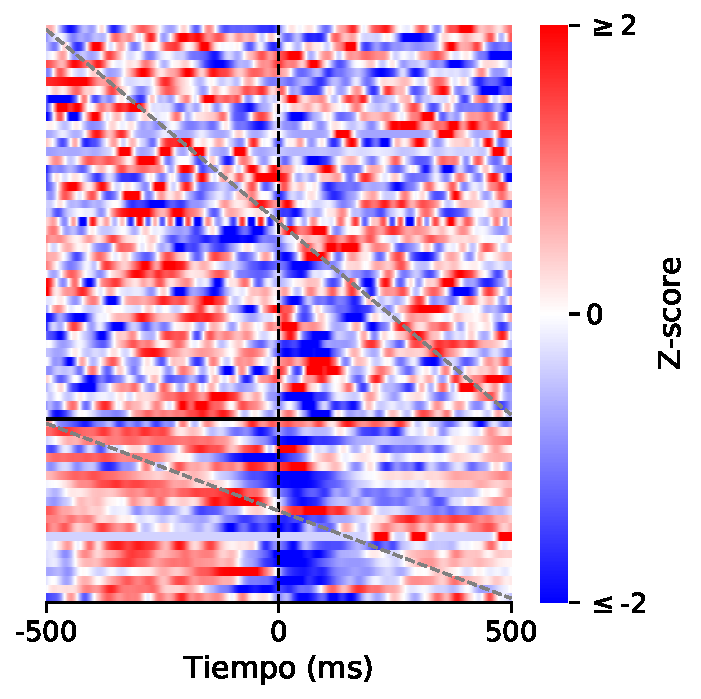
\includegraphics[width=0.53\textwidth]{figuras/expertos/zscore/rasters_separate_days_zscore_deafult_offset_label2.pdf}}
\end{tabular}
\caption{\textit{Heatmaps} con las respuestas de grupos de neuronas ante la ocurrencia de eventos de transición que involucran al \textit{label} 2. Cada fila de un \textit{heatmap} representa el \textit{z-score} de una única neurona. La actividad de las neuronas están divididas en no moduladas y moduladas. Las actividades de las neuronas se ordenan según la posición de su máximo, mínimo y según un orden por defecto.}
\label{fig:zscore_label2}
\end{figure}

\begin{figure}[!htbp]
\begin{tabular}{clll}
& & \multicolumn{2}{c}{\hspace{-5.5em} \textit{Label} 5} \\
& & \hspace{6em} \textit{Onset} & \hspace{6em} \textit{Offset} \\
\rotatebox[origin=c]{90}{Orden según máximo} & \rotatebox{90}{\hspace{-9em} Moduladas \hspace{2.5em} No moduladas} & \raisebox{-0.5\height}{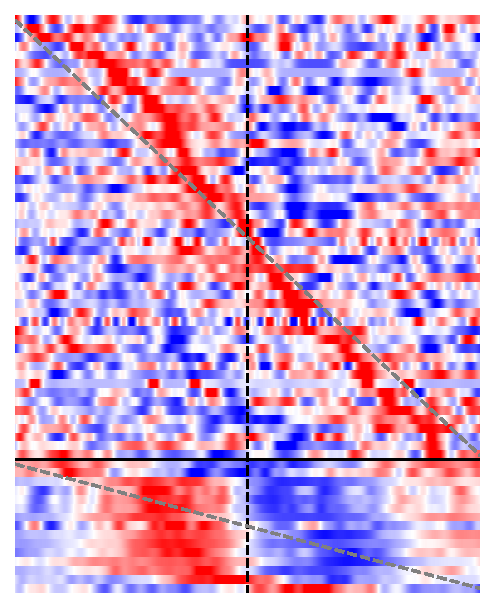
\includegraphics[width=0.37\textwidth]{figuras/expertos/zscore/rasters_separate_days_zscore_max_onset_label5.pdf}} &
\raisebox{-0.5\height}{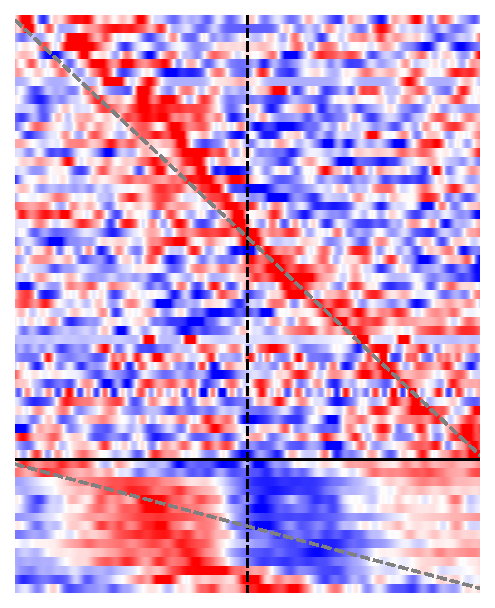
\includegraphics[width=0.37\textwidth]{figuras/expertos/zscore/rasters_separate_days_zscore_max_offset_label5.pdf}} \\
\rotatebox[origin=c]{90}{Orden según mínimo} & & \raisebox{-0.5\height}{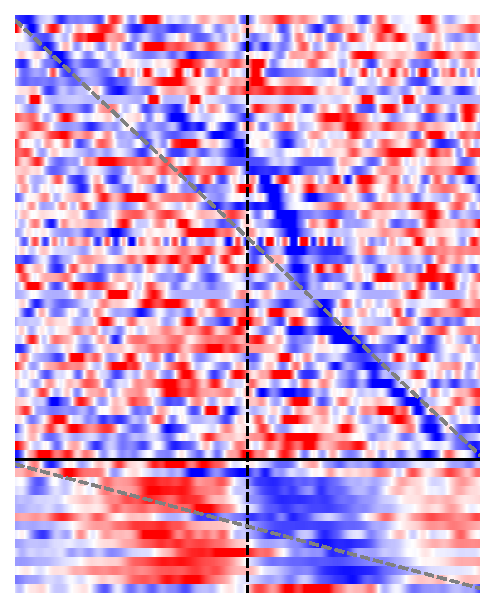
\includegraphics[width=0.37\textwidth]{figuras/expertos/zscore/rasters_separate_days_zscore_min_onset_label5.pdf}} &
\raisebox{-0.5\height}{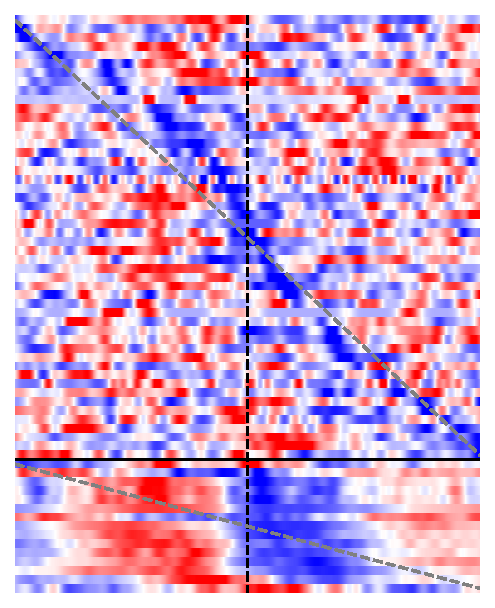
\includegraphics[width=0.37\textwidth]{figuras/expertos/zscore/rasters_separate_days_zscore_min_offset_label5.pdf}} \\
\rotatebox{90}{Orden por defecto} & & \hspace{-1.5em} \raisebox{-0.5\height}{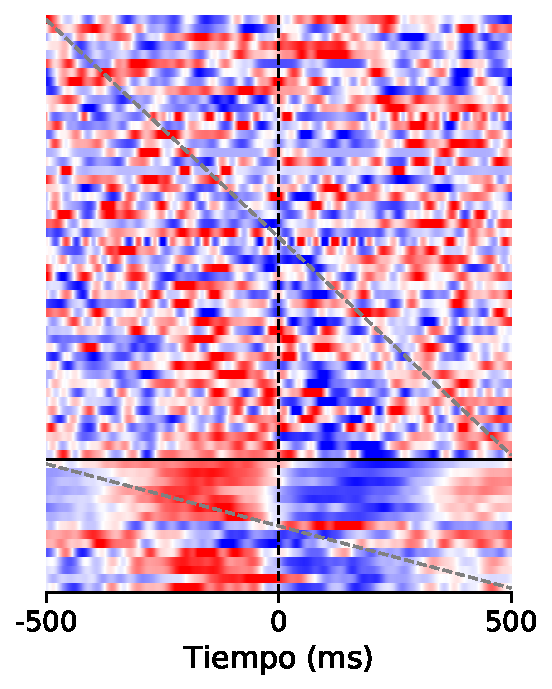
\includegraphics[width=0.42\textwidth]{figuras/expertos/zscore/rasters_separate_days_zscore_deafult_onset_label5.pdf}} & \hspace{-1.3em} \raisebox{-0.495\height}{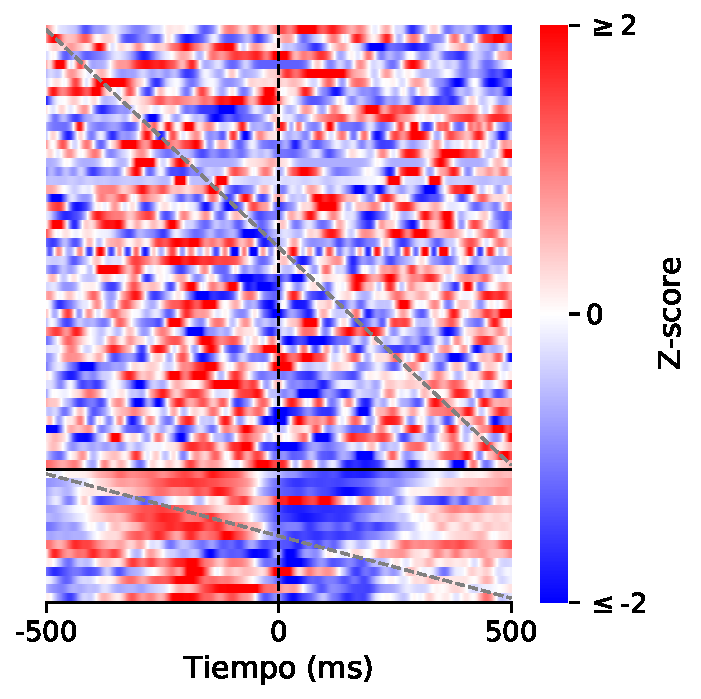
\includegraphics[width=0.53\textwidth]{figuras/expertos/zscore/rasters_separate_days_zscore_deafult_offset_label5.pdf}}
\end{tabular}
\caption{\textit{Heatmaps} con las respuestas de grupos de neuronas ante la ocurrencia de eventos de transición que involucran al \textit{label} 5. Cada fila de un \textit{heatmap} representa el \textit{z-score} de una única neurona. La actividad de las neuronas están divididas en no moduladas y moduladas. Las actividades de las neuronas se ordenan según la posición de su máximo, mínimo y según un orden por defecto.}
\label{fig:zscore_label5}
\end{figure}

\begin{figure}[!htbp]
\begin{tabular}{clll}
& & \multicolumn{2}{c}{\hspace{-5.5em} \textit{Label} 6} \\
& & \hspace{6em} \textit{Onset} & \hspace{6em} \textit{Offset} \\
\rotatebox[origin=c]{90}{Orden según máximo} & \rotatebox{90}{\hspace{-10em} Moduladas \hspace{2.5em} No moduladas} & \raisebox{-0.5\height}{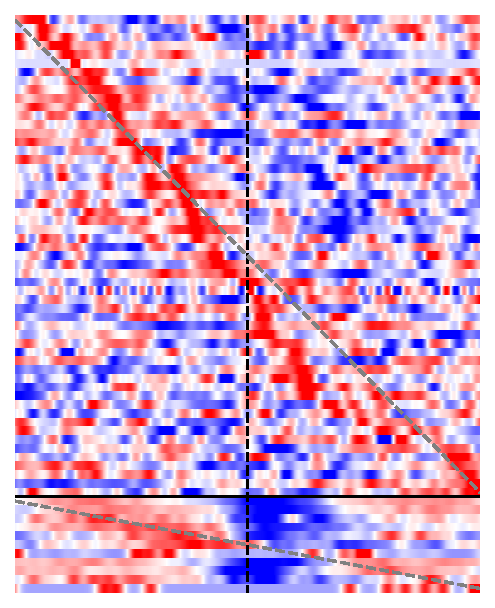
\includegraphics[width=0.37\textwidth]{figuras/expertos/zscore/rasters_separate_days_zscore_max_onset_label6.pdf}} &
\raisebox{-0.5\height}{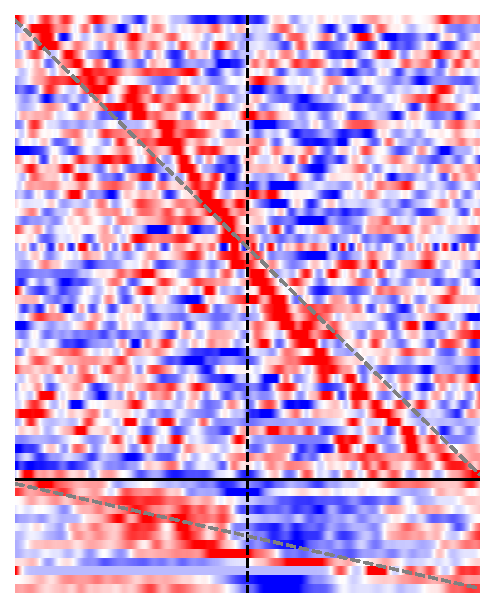
\includegraphics[width=0.37\textwidth]{figuras/expertos/zscore/rasters_separate_days_zscore_max_offset_label6.pdf}} \\
\rotatebox[origin=c]{90}{Orden según mínimo} & & \raisebox{-0.5\height}{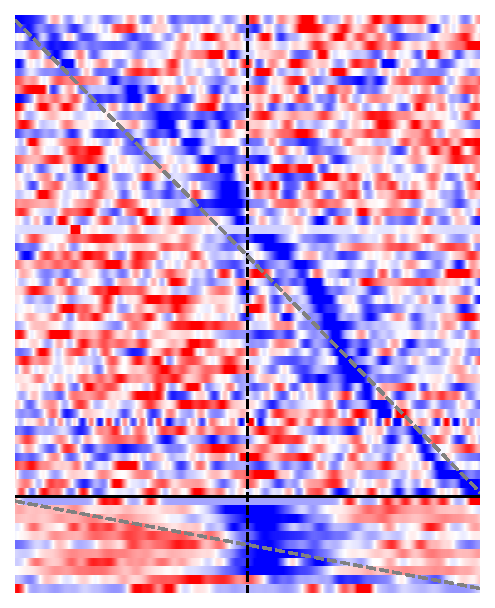
\includegraphics[width=0.37\textwidth]{figuras/expertos/zscore/rasters_separate_days_zscore_min_onset_label6.pdf}} &
\raisebox{-0.5\height}{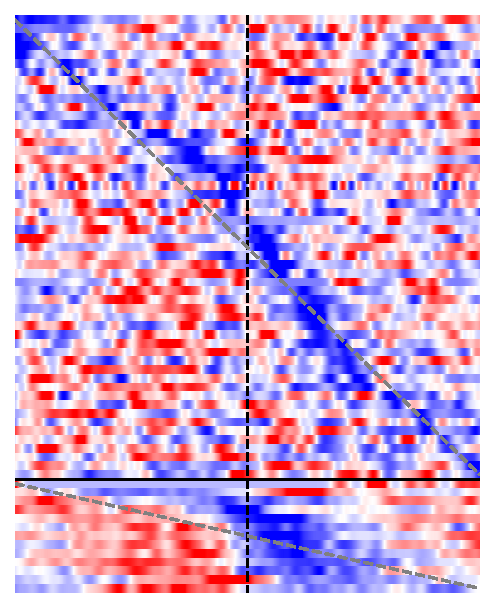
\includegraphics[width=0.37\textwidth]{figuras/expertos/zscore/rasters_separate_days_zscore_min_offset_label6.pdf}} \\
\rotatebox{90}{Orden por defecto} & & \hspace{-1.5em} \raisebox{-0.5\height}{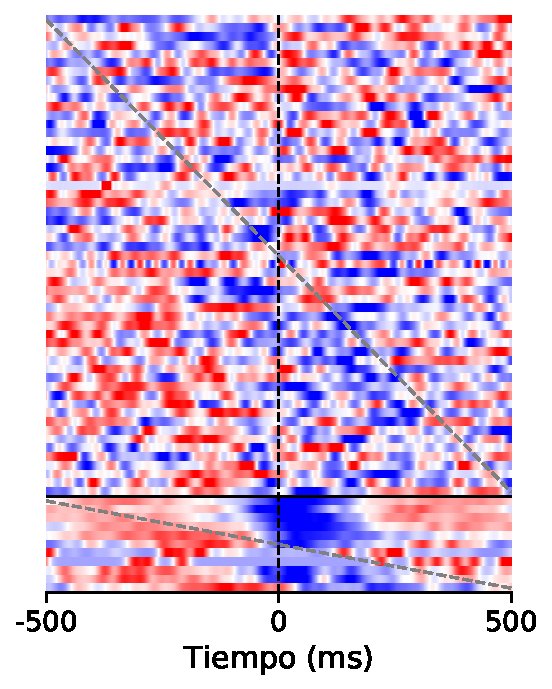
\includegraphics[width=0.42\textwidth]{figuras/expertos/zscore/rasters_separate_days_zscore_deafult_onset_label6.pdf}} & \hspace{-1.3em} \raisebox{-0.495\height}{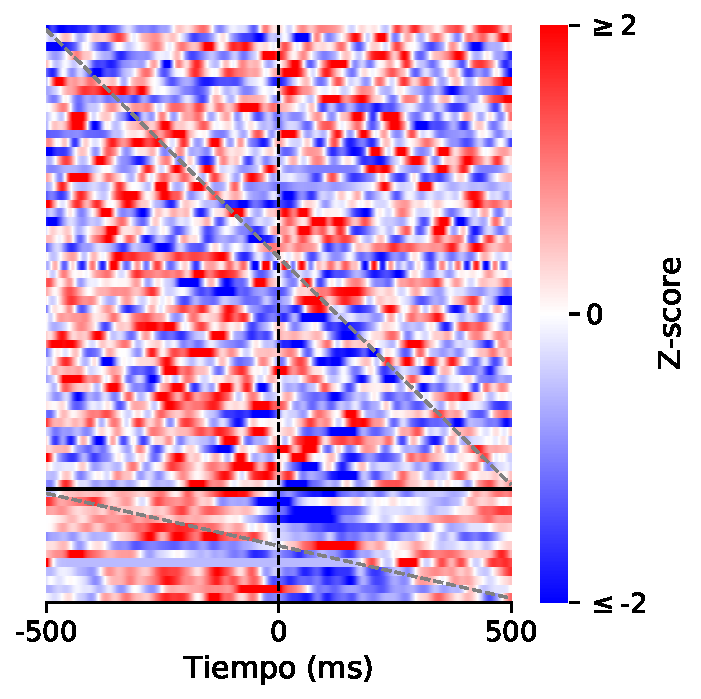
\includegraphics[width=0.53\textwidth]{figuras/expertos/zscore/rasters_separate_days_zscore_deafult_offset_label6.pdf}}
\end{tabular}
\caption{\textit{Heatmaps} con las respuestas de grupos de neuronas ante la ocurrencia de eventos de transición que involucran al \textit{label} 6. Cada fila de un \textit{heatmap} representa el \textit{z-score} de una única neurona. La actividad de las neuronas están divididas en no moduladas y moduladas. Las actividades de las neuronas se ordenan según la posición de su máximo, mínimo y según un orden por defecto.}
\label{fig:zscore_label6}
\end{figure}

\begin{figure}[!htbp]
\begin{tabular}{clll}
& & \multicolumn{2}{c}{\hspace{-5.5em} \textit{Label} 7} \\
& & \hspace{6em} \textit{Onset} & \hspace{6em} \textit{Offset} \\
\rotatebox[origin=c]{90}{Orden según máximo} & \rotatebox{90}{\hspace{-9.5em} Moduladas \hspace{2.5em} No moduladas} & \raisebox{-0.5\height}{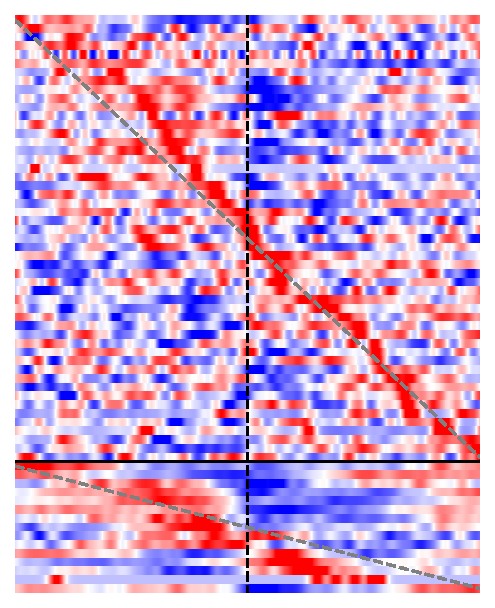
\includegraphics[width=0.37\textwidth]{figuras/expertos/zscore/rasters_separate_days_zscore_max_onset_label7.pdf}} &
\raisebox{-0.5\height}{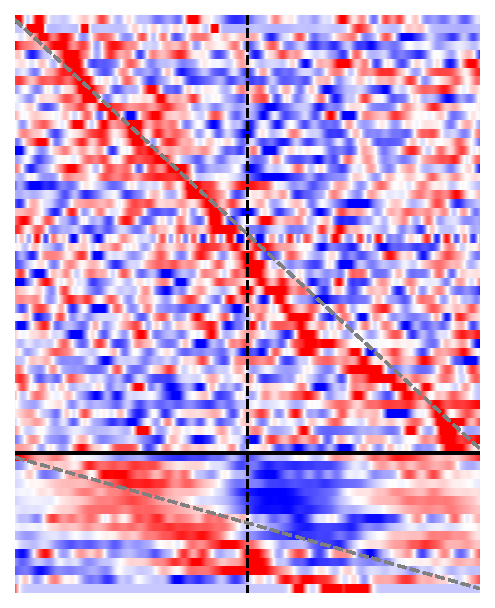
\includegraphics[width=0.37\textwidth]{figuras/expertos/zscore/rasters_separate_days_zscore_max_offset_label7.pdf}} \\
\rotatebox[origin=c]{90}{Orden según mínimo} & & \raisebox{-0.5\height}{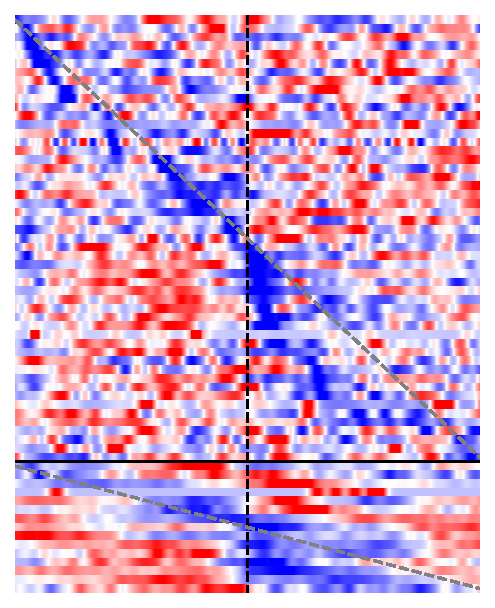
\includegraphics[width=0.37\textwidth]{figuras/expertos/zscore/rasters_separate_days_zscore_min_onset_label7.pdf}} &
\raisebox{-0.5\height}{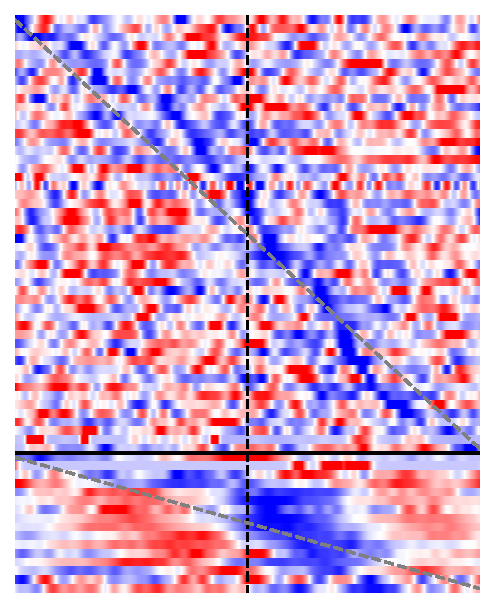
\includegraphics[width=0.37\textwidth]{figuras/expertos/zscore/rasters_separate_days_zscore_min_offset_label7.pdf}} \\
\rotatebox{90}{Orden por defecto} & & \hspace{-1.5em} \raisebox{-0.5\height}{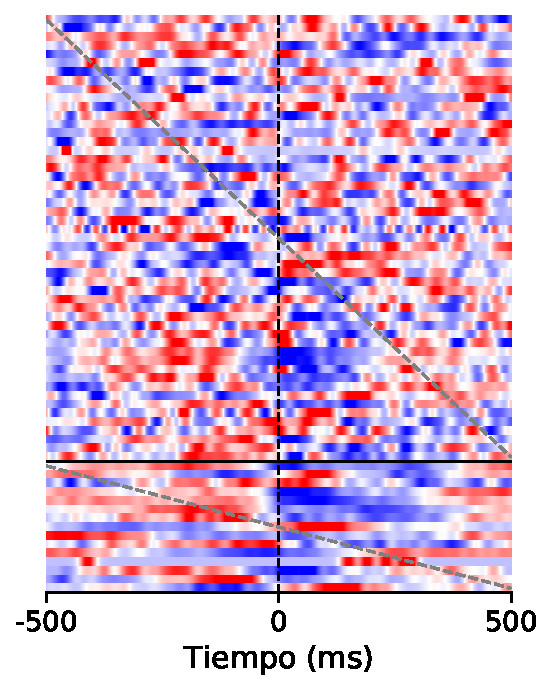
\includegraphics[width=0.42\textwidth]{figuras/expertos/zscore/rasters_separate_days_zscore_deafult_onset_label7.pdf}} & \hspace{-1.3em} \raisebox{-0.495\height}{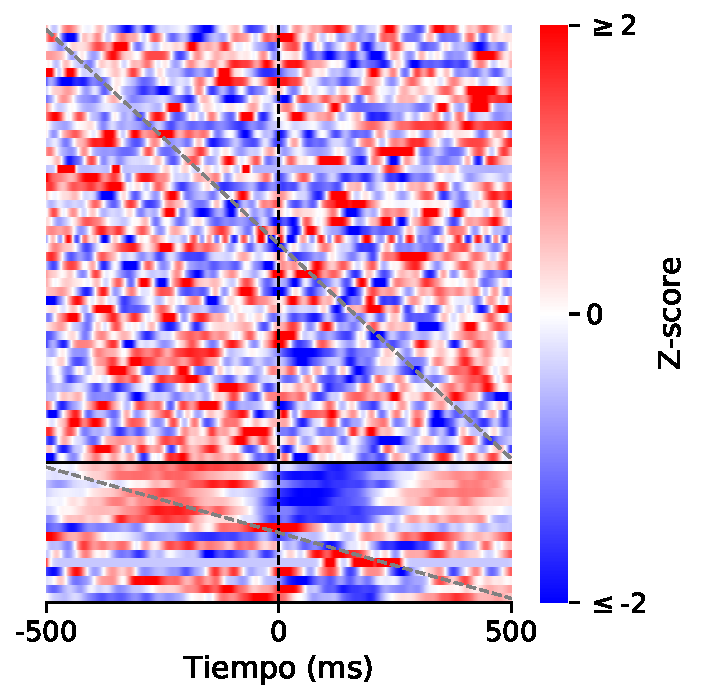
\includegraphics[width=0.53\textwidth]{figuras/expertos/zscore/rasters_separate_days_zscore_deafult_offset_label7.pdf}}
\end{tabular}
\caption{\textit{Heatmaps} con las respuestas de grupos de neuronas ante la ocurrencia de eventos de transición que involucran al \textit{label} 7. Cada fila de un \textit{heatmap} representa el \textit{z-score} de una única neurona. La actividad de las neuronas están divididas en no moduladas y moduladas. Las actividades de las neuronas se ordenan según la posición de su máximo, mínimo y según un orden por defecto.}
\label{fig:zscore_label7}
\end{figure}